
\documentclass{../download/tPRS2e}

\usepackage{tikz}
\usetikzlibrary{patterns}
\usepackage{graphicx}
\graphicspath{{media/}}

\begin{document}

\title{Some Optimization Models of Tool Path Problem for Sheet Cutting Machines}

\author{
\name{
Petunin A.A.\textsuperscript{a},
Chentsov P.A.\textsuperscript{b}\textsuperscript{a},
Polishuk E.G.\textsuperscript{a},
Ukolov S.S.\textsuperscript{a}$^{\ast}$\thanks{$^\ast$Corresponding author. Email: s.s.ukolov@urfu.ru}
}
\affil{\textsuperscript{a}Ural Federal University, Yekaterinburg, Russia;
\textsuperscript{b}Institute of Mathematics and Mechanics, Ural Branch of the Russian Academy of Sciences, Yekaterinburg, Russia}
}

\maketitle

\begin{abstract}
TODO
\end{abstract}

\begin{keywords}
    thermal cutting;
    discrete optimization;
    toolpath routing;
    technological constraints;
    dynamic programming;
    thermal deformations
\end{keywords}

\section{Introduction}

The problem of cutting tool path optimization
is one of the applied optimization problems arising
in the design of control programs for CNC plate cutting machines.
The cost or time spent is typically used
as objective function to optimize.
The control program is generated by special software 
(Computer-Aided Manufacturing, CAM-system)
just after another well-known optimization problem
has been solved,
i.e. the problem of nesting
(optimal placement of parts to manufacture on the plate).
The task is to minimize the consumption of sheet material
to produce the parts of known shapes, sizes and quantity.
The example of nesting of 24 parts bounded by 30 closed contours
in rectangular area with minimal distance specified is at Fig. \ref{nesting}.
This nesting was obtained by means of Integrated CAD / CAM ``Sirius''.

\begin{figure}[h]
    \begin{center}
    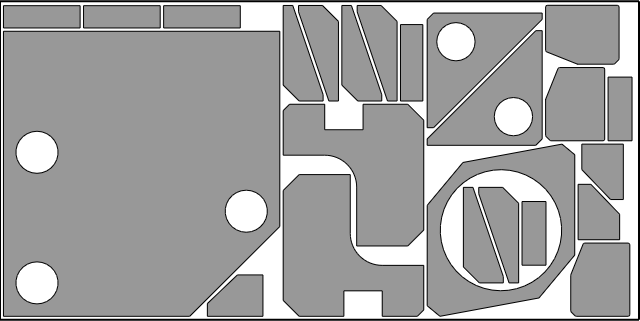
\includegraphics{nesting.png}
    \caption{Example of nesting to a sheet of $2000 \times 1000$ mm
    with minimal distance of $10$ mm} \label{nesting}
    \end{center}
\end{figure}

The process of figure plate cutting with a CNC machine includes
the following activities:
\begin{itemize}
    \item{Pierce point} (cutting start)
    \item{Actual cutting}
    \item{Turning the cutter off} (cutting end)
    \item{Linear movement from end of cut to start of next cut} (air move)
\end{itemize}

Control program usually starts with an air move from
some starting point. Fig. \ref{toolpath} represents
the scheme of cutting two parts with three pierce points.

\begin{figure}[h]
\begin{center}
\tikz{
    \draw[thick,pattern=north east lines, pattern color=gray,even odd rule, rounded corners=2mm]
        (0, 0) ellipse (3 and 2)
        (-2, -1) rectangle (2, 1);
    \draw[thick,pattern=north east lines]
        (7, -1) ellipse (3 and 2);
    \draw[thick]
        (-3, -3) circle(0.05) node[right] {Start of control program};
}
\caption{Example of cutting tool path for two parts and three pierce points} \label{toolpath}
\end{center}    
\end{figure}

The above figure shows tool path going
along the boundary contours of parts,
while in real life it should be offset to
a half cut width in order to preserve parts geometry and sizes.
From the other hand,
most CAM software assume
the path of cutting tool goes
along parts boundaries,
and actual shift is calculated
by CNC machine itself
or special postprocessing software
while converting tool path
from CAM internal representation
to specific CNC machine language.
In the former case,
exact value of cut allowance
is set by CNC machine operator
just before cutting process.
We will further assume
(if not specified otherwise)
that cutting head path is programmed
directly along bounding contours of the parts to cut,
and final tool path contains all the parts contours.
Due to certain technological requirements
pierce points must lay at some extra distance
from part boundaries.
This leads to appearing of additional component,
named ``lead-in''.
In general,
the point of tool switching off
often lay at some
(another) distance from contour to cut,
the resulting tool path addition
is named ``lead-out''
that goes from part boundary to the cut end.
Sometimes lead-out length is allowed to be zero,
causing cutter head to be switched off
directly at the just cut contour.

Let us introduce some notation for tool path components.

We denote $A_1, A_2, \dots A_n$ -- two-dimensional shapes
(closed sets)
that are single- or multiple-connected
regions of Euclidean plane
$\mathbb R^2$.
They are bounded by one or several closed curves
(bounding contours)
$C_1, C_2, \dots C_N,
A_i, C_j \subset \mathbb R^2,
i \in \overline{1, n},
j \in \overline{1, N},
n \leqslant N)$.
Objects $A_1, A_2, \dots A_n$
represent plain parts to cut.

Let also define plane area
$B \subset \mathbb R^2$,
the model of 
sheet material, from which parts are to be cut out.
In general,
this area can be of arbitrary complex shape
(contain several non-rectangular pieces),
but in context of tool path optimization
we will assume it to be
one closed point set bounded
(as well as a detail) by one outer contour.
The holes
(inner contours) are acceptable either.
We will suppose the nesting
(positon of the parts within $B$)
somehow fixed already,
meeting the condition of
mutual non-inersection.
Some other requirements may also arise
due to specific technlogical features
of CNC equipment used.
Any way,
fixed disposition of
$A_1, A_2, \dots A_n \subset B$
is available to us.

Then we denote $S=MM^*$ -- a cutting segment,
i.e. the path of cutting head
from pierce point $M$
to the corresponding cut end point $M^*$.
In terms of geometry,
cutting segment is a curve at Euclidean plane:
$S \subset \mathbb R^2,
M(x,y) \in \mathbb R^2,
M^*(x^*,y^*) \in \mathbb R^2$.
We suppose
the cut direction is defined
in every point of segment $S$.
In case when there are no
closed loops inside segment,
cut direction at each point of segment
is defined uniquely by the starting
point of segment $M$
(pierce point).
Tool path can contain closed loops
not only as part bounding contours,
but also to improve cutting quality.

Using the notion of cutting segment,
all the CNC machine cutting technics
can be classified as:
\begin{enumerate}
    \item{\textit{Closed contour cutting (standard)}}:
    each segment contains exactly one part contour
    that is cut from start to end
    \item{\textit{Multi-segment cutting}}:
    part contour consists of two (or more) cutting segments
    \item{\textit{Multi-contour cutting}}:
    several part contours are cut at once within one cutting segment
\end{enumerate}

For instance, Fig. \ref{toolpath}
shows cutting path with only
standard cutting used.
Example of multi-contour cutting is at
Fig. \ref{cutting},
it uses nesting from Fig. \ref{nesting}.
There are 24 parts on the sheet.
Three groups of thermalhave been cut with multi-contour cutting:
$M1$ (3 parts),
$M7$ (4 parts) and
$M11$,
marked brown.
All other contours have been cut
with ctandard cutting technique.
Parts are cutted in the order of
pierce points $M_j, j=1, 2, \dots 24$.
Return to starting point $M_0$
after cutting is skipped.

\begin{figure}[h]
    \begin{center}
    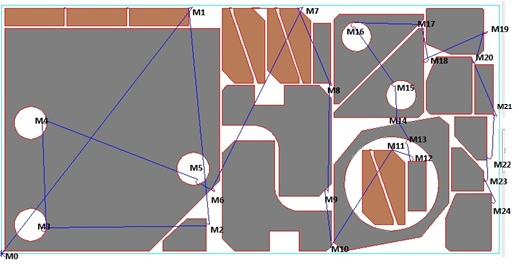
\includegraphics{cutting.png}
    \caption{Example of cutting path with 24 cutting segments} \label{cutting}
    \end{center}
\end{figure}

Let's suppose that our parts
($A_1, A_2, \dots A_n$) were cut
using $K$ cutting segments
$S_k = M_kM_k^*, k \in \overline{1, K}$.
Then we define cutting path as tuple
\begin{equation}
    ROUTE = 
    \left< M_0, M_1, S_1, M_1^*, M_2, S_2, M_2^*, \dots, M_K, S_K, M_K^*, i_1, i_2, \dots, i_K\right>
    \label{tuple}
\end{equation}
Here $i_1, i_2, \dots, i_K$ is the sequence of segments
$S_1, S_2, \dots S_K$ processing,
$M_0$ -- starting point of control program.
Linear air moves are impicitly defined by the tuple.
In terms of discrete mathematics,
the sequence is a permutation,
i.e. an ordered set of natural numbers $1\dots K$,
that unambiguously maps every
$K \in \overline{1, K}$ to $i_k$.
As noted before,
we assume tool path to go along
bounding contours of parts
and cutting segments to contain all of them:
$$
\bigcup_{j=1}^N C_j \subset \bigcup_{k=1}^K S_k
$$
Modifying cutting path one can
drastically change numerical parameters
of cutting process.
Therefore a number of optimization problems
arise while developing
control programs for CNC cutting machines.
The most popular objective function
is total cutting time.
In case of thermal or 
hydrobarasive cutting the following formaula applies:
\begin{equation}
    T_{cut} = \frac{L_{on}}{V_{on}} + \frac{L_{off}}{V_{off}} + N_{pt} \cdot t_{pt}
    \label{cut-time}
\end{equation}
Here,
$L_{off}$ is total length of air moves,
$L_{on}$ is total length of cutting segments,
$V_{off}$ is the speed of air move,
$V_{on}$ is the speed of cutting,
$N_{pt}$ is the number of pierce points,
$t_{pt}$ is the time spent in a pierce point,
assuming it is located in the body of sheet.
In some scenarios other kinds of pierce points
can be used
with their own $t_{pt}$ constants.
In that case, equation (\ref{cut-time})
transforms to
\begin{equation}
    T_{cut} = \frac{L_{on}}{V_{on}} + \frac{L_{off}}{V_{off}}
    + \sum_{j=1}^p N_{pt}^j \cdot t_{pt}^j
    \label{piercings}
\end{equation}
Here,
$p$ is a number of pierce point kinds,
$N_{pt}^j$ -- a number of pierce points of kind $j$,
$t_{pt}^j$ -- time to pierce point of kind $j$.
Both in (\ref{cut-time}) and (\ref{piercings}),
$V_{off}$ is a constant dependent on CNC machine used.
Value of $V_{on}$ is to be determined along with
control program development
concerning cutting technology to use
and parameters of sheet material
(including its thickness).
Thus defined $V_{on}$
is often assumed to be a constant value,
but in practice
actual cutting speed depends on
many technological features as well as 
control program itself.
Additional research is required in this area,
some results can be found in [3],
but this is beyond of scope of this article.

Total cost of cutting is another very important
objective function,
especially from economical point of view.
This is rather complex indicator dependent on
electric power consumption,
expendables,
CNC machine maintenance
as well as other operational expenses.

Note that in general cutting cost is not 
proprtional to cutting time,
since it also depends on cutting modes.
It can be estimated like in (\ref{cut-time}):
\begin{equation}
    F_{cost} = L_{on}\cdot C_{on} + L_{off}\cdot C_{off} + N_{pt} \cdot C_{pt}
    \label{cut-cost}
\end{equation}
Where
$C_{on}$ is the unit cost of cutting,
$C_{off}$ is that of air move and
$C_{pt}$ is the cost of a piercing a point,
while $L_{on}, L_{off}$ and $N_{pt}$
make the same sence as in (\ref{cut-time}).
Exact values of unit costs
$C_{on}, C_{off}$ and $C_{pt}$
depend on CNC equipment, cutting technology,
sheet material and its thickness.
This dependency is usually summarized
in tabular form or even analitically.

In its turn,
the task of finding appropriate unit costs
$C_{on}, C_{off}$ and $C_{pt}$
for specific equipment and material 
is  low-studied itself.
[4] contains some data concerning this problem
for cutting carbon and stainless stell
as well as aluminium and its alloys
with laser CNC machine ByStar 3015.

When different pierce technologies are used,
(\ref{cut-cost}) becomes
\begin{equation}
    F_{cost} = L_{on}\cdot C_{on} + L_{off}\cdot C_{off}
    + \sum_{j=1}^p N_{pt}^j \cdot C_{pt}^j
    \label{piercings-cost}
\end{equation}
using $C_{pt}^j$ for
cost of piercing of kind $j$.

In any case,
the value of above objective function
depends entirely on the tuple (\ref{tuple})
elements,
i.e. the cutting path.
In detail,
the geometry of cutting segments
$S_1, S_2, \dots S_K$ gives us
total cutting length $L_{on}$,
while points $M_0, M_1, M_1^*, \dots M_K, M_K^*$
with permutation $i_1, i_2, \dots i_K$
describe air moves hence its total length $L_{off}$.

Therefore,
mentioned above problems
of cutting path optimizations may be
stated as minimization of some objective function $F$,
defined on set $G$ of addmisible tuples (\ref{tuple}):
\begin{equation}
    F(ROUTE) \to \min_{ROUTE \in G}
    \label{minimize}
\end{equation}
As tuple contains both
cutting sequence 
$i_1, i_2, \dots i_K$
and cutting start and end points 
$M_kM_k^*, k \in \overline{1, K}$,
the latter located on the Euclidean plane $\mathbb R^2$,
general optimization problem (\ref{minimize})
is a very complex 
continuous-discrete optimization problem,
even with significant restrictions imposed
on admissible segments
$S_1, S_2, \dots S_K$.

This leads to the fact that
there are no general algorithms for solving the problem (\ref{minimize})
described in the scientific literature. 
Nevertheless,
some narrow classes of problems
exist,
that allow efficent optimization algorithms to be developed.
We mention four such classes [4-6].

\begin{enumerate}
    \item{\textbf{Continuous Cutting Problem (CCP)}}:
    the cutter head visits each contour to be cut once.
    The tool can engage the contour at any point on its perimeter,
    but must cut the entire
    contour before it travels to the next contour.
    Accordingly, the same point must be used for
    entry and exit the contour.
    In terms of cutting techniques CCP implies the standard one.
    With no constraints on the pierce points,
    problem (\ref{cut-time}) reduces to finding minimal
    air move distance $L_{off}$,
    which is equivalent to the classical metric TSP
    (Travelling Salesman Problem).
    A significant part of the publications is devoted precisely
    to the solution of this particular optimization problem
    \item{\textbf{Endpoint Cutting Problem (ECP)}}:
    the tool can enter and exit contours only at some
    predefined points on the boundary.
    However, it may cut the contour in sections,
    or stated otherwise: a contour can be pre-empted.
    This approach reduces the complexity of full problem
    by discretiztion of possible pierce point set and therefore
    contour entry points as well.
    Set of contour exit points is equal to that of
    entry points, however,
    contour exit point is not neccesary
    a point of cutting end 
    (where cutting head is switched off),
    because cutting can continue to another contour.
    \item{\textbf{Generalized Traveling Salesman Problem (GTSP)}}:
    the tool path visits each contour to be cut once
    and the tool can engage the contour only
    at some predened points on the boundary.
    This is a special case for CCP and ECP problems.
    \item{\textbf{Segment Continuous Cutting Problem (SCCP)}}:
    cutter head visits each segment to be cut once.
    The tool can engage the segment at any point,
    but must cut the entire segment before it travels to the next segment.
    Note: $CCP \subset SCCP$.

    This case uses the concept of basic cutting segment
    (see [3])
    $B^S$, the part of full cutting segment
    $S = MM^*$ with lead-in and lead-out excluded.
    Unlike full cutting segments,
    basic ones doesn't assume cutting direction,
    containig only geometrical data.
    When standard cutting technique is used only,
    the set of basic segments $\cup B^S = \cup C_i$
    (the set of bounding contours).
\end{enumerate}

Most publications on the area explore GTSP problem
and develop appropriate algorithms.
Its main advantage is that most methods
of standard GTSP problems can be applied,
only some additional constraints should be
taken into account,
for instance -- precedence constraint.

It imposes restrictions on the order of
segment processing
$I = (i_1, i_2, \dots i_K)$.
Modern CNC cutting equipment cannot guarantee
positioning of cutting head inside the contour
that is alredy cut,
because the part can freely move 
(or even drop)
after it is detached from the sheet.
To cope with this,
the following rules must be obeyed:

\begin{enumerate}
    \item{If one or more inner contours (holes) are inside outer one,
    then they all must be cut before cutting of outer contour starts
    }
    \item{If some other part is placed inside
    inner contour of a part,
    the former one must be cut before the latter.
    Rule 1 applies either.}
\end{enumerate}
These rules are the precedence constraint
for the permutation
$I = (i_1, i_2, \dots i_K)$.
In other words:
\begin{enumerate}
    \item{If permutation 
    $I = (i_1, \dots i_k, \dots i_K)$
    contains outer contour $i_k$,
    all its corresponding inner contours $i_x$
    must apeear before $i_k$.
    }
    \item{If permutation 
    $I = (i_1, \dots i_k, \dots i_K)$
    contains inner contour $i_k$
    and there is some outer contour
    of another part $A_l, l \in \overline{1,n}$
    inside it,
    that outer contour must precede $i_k$
    in permutation $I$}
\end{enumerate}

Both the precedence constraint
and pierce point constraints
are of static nature,
that is they are completely defined by
the nesting the parts on the sheet,
CNC equipment and material used
and are not affected by the elements
of tuple itself.
In terms of tool path $ROUTE$
(\ref{tuple}),
some of permutations
$I = (i_1, i_2, \dots i_K)$
are just forbidden.
Of many recent papers
on GTSP cutting optimization algorithms,
we note [7-10].

A number of technological features of modern CNC equipment
impose a few other constraints on
pierce points and segment cutting order.
But unlike mentioned above,
these constraints are dynamic,
they depend on the preceding elements
of tuple (\ref{tuple})
and caused by
thermal deformations of sheet material.
It is rather difficult to get comprehensive
equation for such constraints,
see [11,12] for approaches.
These constraints, however,
are also beside the scope of the paper.

Another class of cutting path optimization problems exists,
named \textbf{Intermittent Cutting Problem (ICP)}.
This is the most general version of the problem
where contours can be pre-empted and there is
no restriction on the points that can be used for entry or exit.
It is roughly equivalent to problem (\ref{minimize}).

We are going to explore the approach
that from one hand
extends problems CCP, SCCP and GTSP
and from the other hand
subclasses ICP.
It gives birth to new algorithms for
cutting path optimization.

\section{Dual relaxation}

To solve CCP optimization problem one should find
\begin{enumerate}
    \item{Positions of all pierce point $M_j$} (continous optimization)
    \item{Order of segment processing $I = (i_1, i_2, \dots i_K)$ } (discrete optimization)
\end{enumerate}
minimizing cutting time (\ref{cut-time})
hence air move length $L_{off}$.

Na\"ive but surprisingly well performant approach is to combine
two independent optimizations.

\subsection{Continous optimization}

Assuming permutation 
$I = (i_1, i_2, \dots i_K)$
is fixed somehow,
we are to find pierce point positions for every
cutting segment $S_k$.
We start from arbitrary positions
and relax them one by one,
minimizing total length.

If all but one pierce points are fixed,
finding optimal position for that one 
is rather trivial using Fermat principle,
see Fig. \ref{fermat}.

\begin{figure}[h]
    \begin{center}
    \tikz{
        \draw[thick]
            (0, 0) -- (2, 3) node[right] {$S_k$};
        \fill[black] (0.6666, 1) circle (0.1) coordinate (middle) node[right]  {$M_k \equiv M_k^*$};
        \fill[black] (-2, 0.5) circle (0.1) coordinate (from) node[below]  {$M_{k-1}$};
        \fill[black] (-1, 2.5) circle (0.1) coordinate (to) node[above] {$M_{k+1}$};

        \draw[dashed] (from) -- (middle) -- (to);
    }
    \caption{Optimal pierce point position} \label{fermat}
    \end{center}    
\end{figure}
    
The relaxation is performed for every cutting segment
in sequential or random order.
This is rather fast routine
of asymptotic complexity
$O(K)$.

\subsection{Discrete optimization}

The hard part is to find optimal permutation
$I = (i_1, i_2, \dots i_K)$
which is $O(K!)$
(exponential time).

Luckily,
simple brute force attack seems
to quickly bring us next to optimal solution.
We start from some permutation
(random, or from another optimization algorithm)
and attempt to improve it with the following simple steps:

\begin{enumerate}
    \item{}
    It's practical to test all pairwise permutations of initial one.
    Complexity is $O(C_K^2) = O(K^2)$.
    \item{}
    Triple and quadruple permutation are too numerous
    ($O(K^3), O(K^4)$),
    but we test only part of them,
    i.e. ``local'' permutations
    exchanging only segments that are no farther
    than say 50 steps from each other.
    \item{}
    Circular permutations are also good candidates to test.
    \item{}
    Other heuristics can be easily coined.
\end{enumerate}

Continous optimization is performed for every candidate permutation
and when is gives better
(shorter) path,
it replaces the initial permutation.

Such a simple process quickly converges to near optimal solution.
It can be easily parallelized and many other
modern techniques used to improve performance.

\subsection{Precedence constraint}

It's suprisingly easy to meet precedence constraint in such a process.

We start from removing all segments $S_k$,
that contains other segments inside.
This happily decreases dimension of problem space
hence decreasing time complexity.

Diecrete optimization is performed as described above.
As soon as better solution is found we just
insert outer contours after their corresponding inner ones,
selecting pierce point as the intersection of air moves with
outer contours.
This process is also $O(K)$.

\subsection{Numerical expreriments}

Such a simple algorithm has a pretty good performance
both in terms of speed and solution quality.

\section*{Acknowledgements}

The work was supported by Act 211 Government of the Russian Federation, contract № 02.A03.21.0006

\bibliographystyle{../download/tPRS}
\nocite{*}
\bibliography{en}

\end{document}
